% 12pt .6pt grayscale fragment
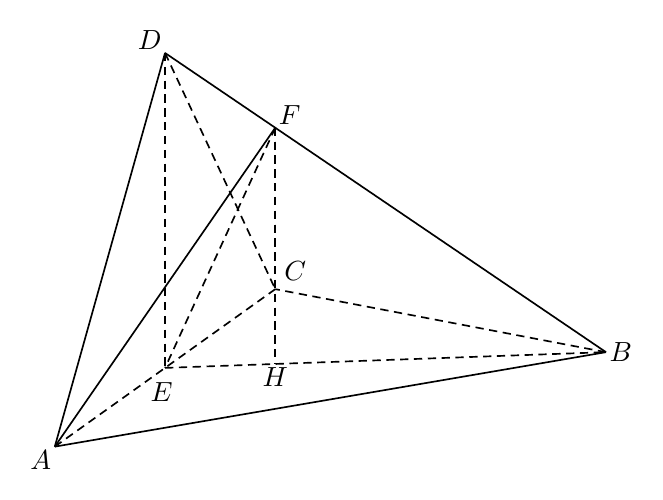
\begin{tikzpicture}[line width=.6pt, font=\normalsize]
\coordinate (A) at (0,0);
\coordinate (B) at (7,1.2);
\coordinate (C) at (2.8,2.0);
\coordinate (D) at (1.4,5);
\coordinate (E) at (1.4,1.0);
\coordinate (F) at (2.8,4.05);
\coordinate (H) at (2.8,1.05);
\draw[densely dashed] (A)--(E)--(C);
\draw[densely dashed] (B)--(C);
\draw[densely dashed] (D)--(C);
\draw[densely dashed] (D)--(E);
\draw[densely dashed] (E)--(H)--(B);
\draw[densely dashed] (F)--(C);
\draw[densely dashed] (F)--(E);
\draw[densely dashed] (F)--(H);
\draw (A)--(D);
\draw (A)--(B);
\draw (A)--(F);
\draw (D)--(F)--(B);
\node[below left,inner sep=1pt] at (A) {$A$};
\node[right,inner sep=1pt] at (B) {$B$};
\node[above right=2pt,inner sep=1pt] at (C) {$C$};
\node[above left,inner sep=1pt] at (D) {$D$};
\node[below left,inner sep=1pt,xshift=4.00bp,yshift=-4.00bp] at (E) {$E$};
\node[above right,inner sep=1pt] at (F) {$F$};
\node[below,inner sep=1pt] at (H) {$H$};
\end{tikzpicture}
